% !TeX spellcheck = pl_PL
\documentclass[a4paper,twoside]{article}
\usepackage{polski}
\usepackage[utf8]{inputenc}
\usepackage[pdftex]{graphicx}
\usepackage{amsmath}

\usepackage[unicode, bookmarks=true]{hyperref} %do zakładek
\usepackage{tabto} % do tabulacji
\NumTabs{11} % globalne ustawienie wielkosci tabulacji
\usepackage{array}
\usepackage{multirow}
\usepackage{array}
\usepackage{dcolumn}
\usepackage{bigstrut}
\usepackage{color}
\usepackage[usenames,dvipsnames]{xcolor}
\usepackage{pdfpages}
\usepackage{sidecap}
\usepackage{wrapfig}
\usepackage{float}	%for figure& table placement in text
\usepackage{textgreek}

\usepackage{listings}
\usepackage{xcolor}
\usepackage{hyperref}
\usepackage{endnotes}

\lstdefinestyle{sharpc}{language=[Sharp]C, frame=lr, rulecolor=\color{blue!80!black}}

\lstdefinelanguage{CSharp}
{
	morecomment = [l]{//}, 
	morecomment = [l]{///},
	morecomment = [s]{/*}{*/},
	morestring=[b]", 
	sensitive = true,
	morekeywords = {abstract,  event,  new,  struct,
		as,  explicit,  null,  switch,
		base,  extern,  object,  this,
		bool,  false,  operator,  throw,
		break,  finally,  out,  true,
		byte,  fixed,  override,  try,
		case,  float,  params,  typeof,
		catch,  for,  private,  uint,
		char,  foreach,  protected,  ulong,
		checked,  goto,  public,  unchecked,
		class,  if,  readonly,  unsafe,
		const,  implicit,  ref,  ushort,
		continue,  in,  return,  using,
		decimal,  int,  sbyte,  virtual,
		default,  interface,  sealed,  volatile,
		delegate,  internal,  short,  void,
		do,  is,  sizeof,  while,
		double,  lock,  stackalloc,   
		else,  long,  static,   
		enum,  namespace,  string}
}

\let\footnote=\endnote

\setlength{\textheight}{24cm}
\setlength{\textwidth}{15.92cm}
\setlength{\footskip}{10mm}
\setlength{\oddsidemargin}{0mm}
\setlength{\evensidemargin}{0mm}
\setlength{\topmargin}{0mm}
\setlength{\headsep}{5mm}
\newcommand{\HRule}{\rule{\linewidth}{0.5mm}} 

\newcolumntype{M}[1]{>{\centering\arraybackslash}m{#1}}
\newcolumntype{N}{@{}m{0pt}@{}}

\graphicspath{ {./img/} }

% === Reset inkrementacji sekcji przy nowym parcie === %
\usepackage{titlesec}

\makeatletter
\@addtoreset{section}{part}
\makeatother
\titleformat{\part}[display]
{\normalfont\LARGE\bfseries\left}{}{0pt}{}

\titleformat{\chapter}[hang]{\LARGE\bfseries}{\thechapter\hsp\textcolor{blue}{|}\hsp}{0pt}{\Huge\bfseries}


\begin{document}
	
	\begin{titlepage}
		\begin{center}
			
			% Upper part of the page. The '~' is needed because \\
			% only works if a paragraph has started.
			
\includegraphics[width=0.5\textwidth]{./img/logo.png}~\\[1cm]
			%?[width=0.15\textwidth]
			
			\textsc{\LARGE Politechnika Śląska w Gliwicach}\\[1.5cm]
			
			\textsc{\LARGE Biologically Inspired Artificial Intelligence}\\[0.2cm]
			
			\textsc{\LARGE Raport z projektu}\\[0.2cm]
			
			% Title
			\HRule \\[0.4cm]
			{ \Huge \bfseries Predykcja jakości obrazów na podstawie metadanych \\[0.4cm] }
			
			\HRule \\[1.5cm]
			
			% Author and supervisor
			\textsc{\Large Autorzy:} \\
			Bartłomiej Buchała \\
			Marek Motyka \\[1.0cm]
			
			Informatyka, semestr VI \\
			Rok akademicki 2014/2015 \\
			Grupa GKiO3
			
			\vfill
			
			% Bottom of the page
			{\large \today}
			
		\end{center}
	\end{titlepage}
	
\newpage

\section{Temat projektu}

Naszym głównym zagadnieniem projektowym z przedmiotu Biologiczne Motywowane Metody Sztucznej Inteligencji została predykcja jakości obrazów na podstawie metadanych. Problematyka ta jest przedmiotem jednego z wielu tematów konkursowych na stronie konkursowej kaggle.com \footnote{\url{https://www.kaggle.com/c/PhotoQualityPrediction}}. \\

Podstawową jednostką danych był album zdjęć - każdy z nich posiadał zestaw kolumn zawierający zestaw informacji o zdjęciach do niego należących:

\begin{itemize}
	\item Id - unikatowy identyfikator albumu.
	\item Długość i szerokość geograficzna (\textit{longitude, latitude})- zaogrąglone do liczb całkowitych wartości w stopniach, określające przybliżoną lokację na kuli ziemskiej, w której zostały zrobione zdjęcia.
	\item Wysokość i szerokość (\textit{height, width})- wymiary (w pikselach) znajdujących się w albumie zdjęć.
	\item Wielkość (\textit{size}) - wartość określająca ilość zdjęć w albumie.
	\item Nazwa (\textit{name}) - Lista często powtarzających się w nazwie znaków/ciągów znaków 
	\item Opis (\textit{description}) - Lista często powtarzających się w opisie znaków/ciągów znaków
	\item Podpis (\textit{caption}) - Lista często powtarzających się w podpisie znaków/ciągów znaków
	\item Czy Dobry (\textit{good}) - wartość zerojedynkowa, określająca czy ludzkiemu recenzentowi spodobałby się album. 1 oznacza pozytywną opinię, 0 negatywną.
\end{itemize}

Po rozbiciu na znaki/słowa, tekst zawarty w nazwach, opisach i podpisach został dodatkowo zaszyfrowany w celach anonimowości. Ostatecznie pola w kolumnach \textit{name}, \textit{caption} oraz \textit{description} podane zostały jako listy liczb całkowitych (każda określająca inny znak/ciąg znaków, wyłączając tzw. "Znaki stopu"). \\

Organizator konkursu dostarczył dwa zestawy danych w formacie .csv - treningowy zestaw train.csv posiadający wypełnione informacje w kolumnie \textit{good} oraz zestaw do ewaluacji - test.train nie posiadający informacji o jakości zdjęć albumów.
Naszym zadaniem było wykorzystać algorytm z dziedziny machine learning, aby na podstawie danych treningowych określić czy albumy, których metadane znajdujące się w pliku test.csv, zostałyby pozytywnie ocenione przez ludzkiego ewaluatora. Dane wynikowe również miały być przechowywane w pliku .csv posiadającym tylko 2 kolumny: id albumu oraz ocenę. Zdecydowaliśmy się dodać również możliwość podania przez użytkownika własnych danych - w takim przypadku informacja o przewidywanej jakości albumu ma zostać wyświetlona w głównym oknie aplikacji. \\

Podczas etapu projektowania zdecydowaliśmy się połączyć 2 różne technologie: język programowania C\# wraz z frameworkiem .NET został wykorzystany do stworzenia graficznego interfejsu użytkownika, natomiast do implementacji algorytmu wykorzystaliśmy język R do obliczeń statystycznych. Aby środowisko programistyczne Visual Studio 2012 miał możliwość wykonywania skryptów napisanych w R, konieczne było użycie biblioteki R.NET, pozwalającej tworzyć sesje R w .NET.

\section{Implementacja}

\subsection{Struktura aplikacji}

\subsubsection{Inicjalizacja}

W pierwszej kolejności zajęliśmy się podłączeniem biblioteki R.NET do projektu - bez tego komunikacja pomiędzy skryptami R a .NETEM nie byłaby możliwa. W tym celu stworzona została specjalna klasa powołująca instancję silnika Rengine. Odpowiednie polecenia są wykonywane w metodzie Initialize(); Oprócz utworzenia silnika, biblioteka RDotNet tworzy również nową sesję R, w ramach której przechowywane są zmienne (zarówno wczytane zmienne oraz wyniki obliczeń są usuwane wraz z zakończeniem sesji). Przy zamknieciu aplikacji wywoływana jest metoda engine.Dispose(), pozbywająca się silnika oraz zamykająca sesję (inaczej mogłoby dojść do wycieków pamięci). \\

\newpage

Fragment kodu metody Initialize() odpowiadający za powołanie instancji silnika R:
\lstset{style=sharpc}
\begin{lstlisting}[language=CSharp]
REngine.SetEnvironmentVariables();
engine = REngine.GetInstance();
engine.Initialize();
\end{lstlisting}

\subsubsection{Uruchamianie skryptów}

Ponieważ programy w języku R wykonywane są poprzez interpretowanie pojedynczych poleceń (a nie kompilację całych plików/projektów), zasada posługiwania się nimi przypomina linię poleceń. W celu wywołania algorytmów napisanych w języku R, posługujemy się skryptami - przygotowanymi wcześniej zestawami komend, które wykonywane są jedna po drugiej. Z pomocą przychodzi polecenie source("nazwaPliku"), które pozwala na uruchomienie zagnieżdżonego skryptu w skrypcie. \\

Drugą przydatną instrukcją jest przypisanie do commandArgs polecenia function c("ListaArgumentów"), która pozwala na użycie dowolnej liczby argumentów jako parametrów dla następnego polecenia. Metoda launchScript służy do translacji zmiennych w C\# na parametry wywołania skryptów napisanych w R. W przypadku, gdy konieczne było odczytanie informacji zwrotnej, posłużono się metodą GetSymbol("nazwaZmiennej").

\lstset{style=sharpc}
\begin{lstlisting}
public int launchScript(string scriptName, bool hasArguments,
params string[] arg)
{
 try
  {
    if (engine != null)
    {
     if (hasArguments)
     {
      string arguments = arg[0].ToString();

      for (int i = 1; i < arg.Length; i++)
      arguments += ("," + arg[i].ToString());

      engine.Evaluate("commandArgs <- function() c(" + arguments + ")");                        
     }

     if (scriptName.Contains(".R"))
     engine.Evaluate("source('" + scriptName + "')");
     else
     {
      engine.Evaluate("source('" + scriptName + ".R')");
     }
    }

    if (scriptName.Contains("User"))
    {
     IntegerVector result = engine.GetSymbol("userResult").AsInteger();
     return result[0];
    }

  }
 catch (EvaluationException)
 {
  throw new EvaluationException("Brak pliku");
 }
 return -1;
}
\end{lstlisting}

\subsection{Graficzny interfejs użytkownika}

Program od strony wizualnej nie jest skomplikowany jest to aplikacja jednookienkowa.

\begin{figure}[h]
	\centering
	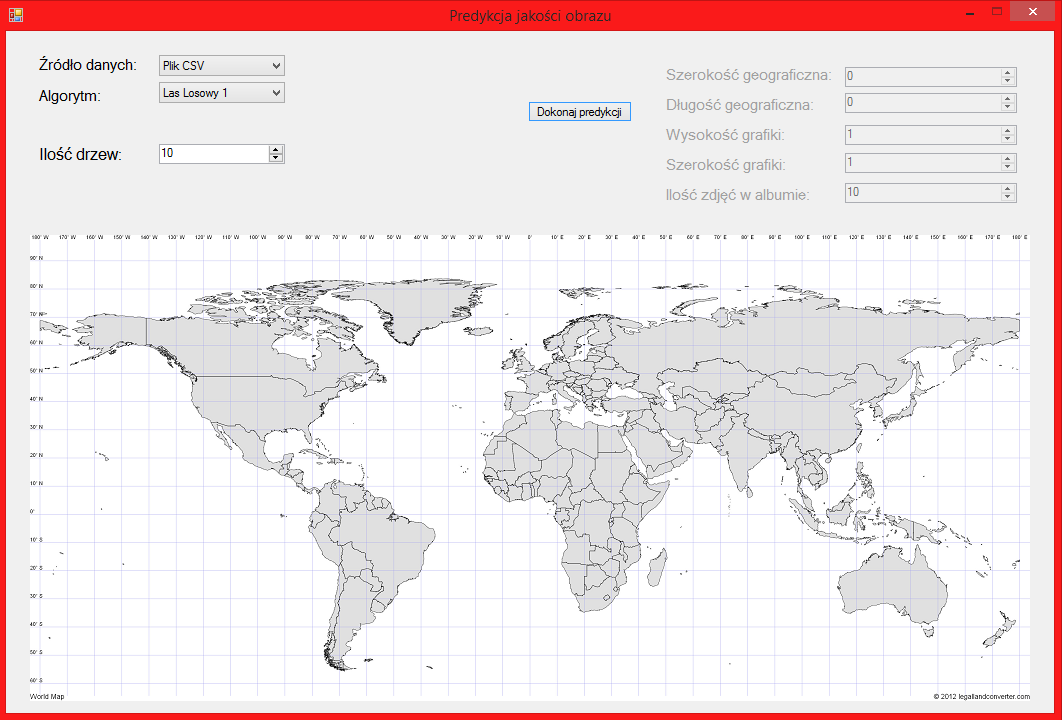
\includegraphics[width=1\textwidth]{./img/001.png}
	\caption{Główne okno aplikacji}
\end{figure}

W lewym górnym rogu dostępne są dwa comboboxy, które pozwalają użytkownikowi wybrać jedną z 2 implementacji algorytmu oraz źródło danych. Przez plik .CSV rozumiany jest dostarczany przez kaggle plik treningowy train.csv, natomiast wybranie opcji "Dane Użytkownika" umożliwia wprowadzenie własnych danych liczbowych do pięciu pól tekstowych znajdujących się w prawym górnym rogu okna.

\begin{figure}[h]
	\centering
	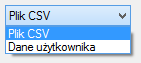
\includegraphics[width=0.2\textwidth]{./img/02.png}
	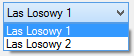
\includegraphics[width=0.2\textwidth]{./img/03.png}
	\caption{Rozwinięte comboboxy}
\end{figure}

W celu zwiększenia atrakcyjności wizualnej programu oraz ułatwienia wprowadzania danych (nie każdy pamięta, na jakiej długości i szerokości geograficznej znajduje się np. Australia), do GUI dodano interaktywną mapę świata. Jeżeli wybrana jest opcja "Dane Użytkownika", kliknięcie na mapę spowoduje wygenerowanie przybliżonych koordynatów dla wybranego obszaru.

\newpage

\begin{figure}[h!]
	\centering
	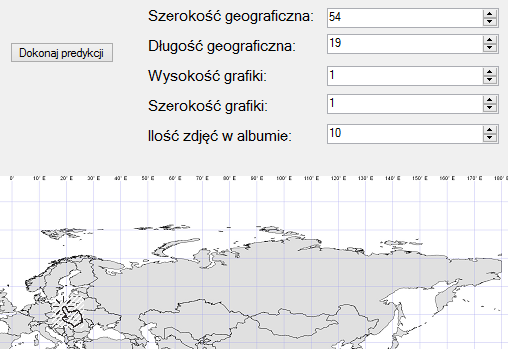
\includegraphics[width=0.5\textwidth]{./img/05.png}
	\caption{Przykład wygenerowania koordynatów po kliknięciu mapy}
\end{figure}

Do generowania lokacji służy poniższy fragment kodu w formularzu MainWindow:

\lstset{style=sharpc}
\begin{lstlisting}
int cursorWidth = pictureBox2.PointToClient(Cursor.Position).X;
int cursorHeight = pictureBox2.PointToClient(Cursor.Position).Y;

float cursorLongitude =
 ((float)cursorWidth / pictureBox2.Width) * 360 - 180;
float cursorLatitude =
 ((float)(pictureBox2.Height - cursorHeight) / pictureBox2.Height)*180-75;

if (comboBox1.SelectedIndex == 1)
 {
   numericUpDown1.Value = (cursorLatitude < 90) ? (int)cursorLatitude : 90;
   numericUpDown2.Value = (int)cursorLongitude;
 }
\end{lstlisting}

\subsection{Algorytm}

\subsubsection{Przygotowanie}

Przy tworzeniu sesji, dane z plików CSV są wczytywane w pliku \textit{setup.R} do tzw. dataframe'ów. Jest to struktura danych przypominająca zwykłą tabelę, posiadjąca jednak parę dodatkowych wbudowanych funkcji ułatwiajacych zarządzanie danymi. Wczytywanie odbywa się poprzez wywołanie funkcji read.csv:

\begin{lstlisting}[language=R]
train <- read.csv("CSV/training.csv", stringsAsFactors = FALSE)
test <- read.csv("CSV/test.csv", stringsAsFactors = FALSE)
\end{lstlisting}

Wykorzystane przez nas algorytmu lasów losowych dokonują predykcji pojedynczego wskazanego przez nas elementu na podstawie atrybutów określonych w tzw. formule. Im więcej atrybutów posiada formuła, tym lepiej - większa ilość pozwala dokonać dokładniejszej estymacji szukanej danej.
W tym celu, dodaliśmy 6 specjalnych kolumn, które będą mogły posłużyć za dodatkowe informacje, według których algorytm lasu będzie określał jakość albumów.

\newpage

\begin{itemize}
	\item Atrybut \textbf{Continent} - określa przynależność do jednej z ośmiu stref (Ameryki Pónocna/Południowa/Środkowa, Azja, Europa, Afryka, Australia, Ocean) na podstawie długości i szerokości geofraficznej. W rzeczywistości, wartości te są przybliżone ze względu na skomplikowany kształt linii brzegowej kontynentów. W naszym modelu określa się prostokąty, w których zawierają się koordynaty danego albumu.
	\item Atrybut \textbf{resolution} - jest w rzeczywistości długością przekątnej zdjęć w albumie. Jest to jedna z wartości pozwalających określić rozmiar zdjęć na ekranie.
	\item Atrybut \textbf{proportions} - przydziela album do jednej z 4 kategorii określających proporcje pomiędzy wysokością, a szerokością zdjęć
	\item Atrybuty \textbf{nameLenght}, \textbf{captionLenght}, \textbf{descriptionLenght} - określają ilość często powtarzających się słów w ramach albumu
\end{itemize}

Dodatkowe kolumny tworzone są w skrypcie \textit{ExtraColumns.R} zarówno dla zestawu \textit{train}, jak i \textit{test}. Poniżej znajduje się część fragmentu kodu zajmującego sie generowaniem dodatkowych atrybutów.

\begin{lstlisting}[language=R]
train$Continent[train$longitude > -168 & train$longitude < -125 &
 train$latitude > 50 & train$latitude < 72] <- 'North America'
train$Continent[train$longitude >  113 & train$longitude < 168 &
 train$latitude > -48 & train$latitude < -12] <- 'Australia'
train$Continent[train$longitude > -10 & train$longitude < 40 &
 train$latitude > 36 & train$latitude < 72] <- 'Europe'
train$Continent[train$longitude > -18 & train$longitude < 35 &
 train$latitude > 5 & train$latitude < 36] <- 'Africa'
[..]
train$proportions[(train$width / train$height) < 1.33] <- '< 4:3'
train$proportions[(train$width / train$height) >= 1.33] <- '4:3'
train$proportions[(train$width / train$height) >= 1.45] <- '3:2'
train$proportions[(train$width / train$height) >= 1.55] <- '> 3:2'
[..]
train$resolution <- as.integer(sqrt(train$height^2 + train$width^2))
\end{lstlisting} 

Ważnym elementem było zadeklarowanie atrybutów \textit{Continent} i \textit{proportions} jako typ factor (podobny do spotykanego w większości języków programowania typu Enumerable) - w przeciwnym wypadku wartości w tych kolumnach byłyby odbierane jako zwykły tekst. W przypadku, gdy jako źródło danych wybrano własne dane, uruchamiany jest również skrypt \textit{LoadUserRecord.R}, który odczytuje dane z linii poleceń, a następnie generuje dodatkowe atrybuty wzorem dal nowego rekordu (podobna procedura jak w \textit{ExtraColumns.R}). \\

\begin{lstlisting}[language=R]
args=(commandArgs())

tmpLongitude = as.integer(args[3])
tmpLatitude <- as.integer(args[2])
tmpHeight <- as.integer(args[4])
tmpWidth <- as.integer(args[5])
tmpSize <- as.integer(args[6])

userInput[1,]$id <- as.integer(1)
userInput[1,]$latitude <- as.integer(tmpLatitude)
userInput[1,]$longitude <- as.integer(tmpLongitude)
userInput[1,]$width <- as.integer(tmpWidth)
userInput[1,]$height <- as.integer(tmpHeight)
userInput[1,]$size <- as.integer(tmpSize)
\end{lstlisting}

\newpage

\subsubsection{Dokonanie predykcji}

Trenowanie lasów oraz generowanie wyników odbywa się w jednym z czterych skryptów (w zależności, jakich ustawień dokonał użytkownik w graficznym interfejsie): \textit{Forest1}, \textit{Forest2}, \textit{UserForest} oraz \textit{UserForest2}. Wszystkie mają podobną budowę i składają się z analogicznych komend:

\begin{enumerate}
	\item Ustawienie generatora liczb losowych - polecenie \textit{set.seed}
	\item Utworzenie lasu losowego za pomocą dołączanych do pakietów poleceń \textit{cforest} lub \textit{randomForest}
	\item Dokonanie predykcji dla danych testowych przy użyciu utworzonego lasu za pomocą polecenia \textit{predict}
	\item Zapisanie uzyskanych danych do nowego dataframe'u i utworzenie z niego pliku wyjściowego
	\item W przypadku "Danych Użytkownika" - pobranie wartości wynikowej i utworzenie zmiennej, do której dostęp będzie miała aplikacja napisana w .NET.
\end{enumerate}

Przykładowy fragment kodu na podstawie skryptu \textit{Forest1}:

\begin{lstlisting}
set.seed(1)
forest1 <- cforest(as.factor(good) ~ Continent + resolution + size
 + latitude + longitude + width + height + proportions + nameLength
  + captionLength + descriptionLength, data=train,
   controls = cforest_unbiased(ntree = 20, mtry = 4))

random_forest_result <- predict(forest1, test, OOB = TRUE, type = "response")
submit <- data.frame(Id = test$id, good = random_forest_result)
write.csv(submit, file = "CSV/random_forest.csv", row.names = FALSE)
\end{lstlisting}

Po wykonaniu wszystkich poleceń otrzymujemy plik wynikowy w folderze "CSV", natomiast w przypadku gdy źródłem są dane użytkownika, zostaje wyswietlona informacja o pozytywnej lub negatywnej ocenie.

\section{Wykorzystane biblioteki}

Do zakodowania algorytmów użyliścmy dwóch różnych pakietów (odpowiedniki bibliotek dla języka R): "randomForest"\footnote{\url{http://cran.r-project.org/web/packages/randomForest/randomForest.pdf}} oraz "party" \footnote{\url{http://cran.r-project.org/web/packages/party/party.pdf}}. Doboru dokonaliśmy na podstawie popularności rozwiązań stosowanych przez uczestników konkursów kaggle'a. \\

Oba pakiety wdrażają algorytm lasów losowych, który z kolei oparty jest na drzewach decyzyjnych (i to na ich poziomie pojawiają się różnice w implementacji). Drzewo decyzyjne jest podobne do drzewiastej struktury danych, gdzie rolę węzłów stanowią miejsca rozszczepienia danych.
W pakiecie "randomForest" Algorytm rozpoczyna swoje działanie w punkcie początkowym, tak zwanym korzeniu ze wszystkimi danymi treningowymi. Następnie przeszukuje wszystkie zmienne (atrybuty), aby wybrać tę, według której najlepiej dokonać podziału. W każdym węźle (za wyjątkiem punktów końcowych - liści) następuje podział na 2 węzły podrzędne. Selekcja dokonywana jest na podstawie "klarowności" (ang. \textit{purity}) węzłów  podzielonych danych - jeden z nich musi mieć jak największy procent jedynek poszukiwanej danej, drugi jak największą ilość zer. Przykładowy fragment takiego drzewa zobrazowany jest poniżej.

\newpage

\begin{figure}[h!]
	\centering
	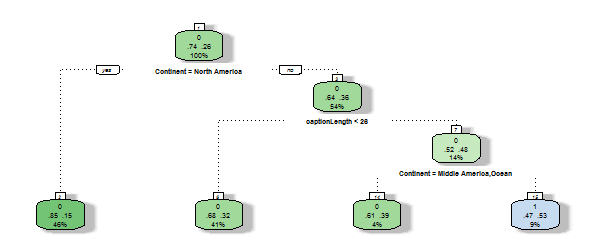
\includegraphics[width=1\textwidth]{./img/Rplot01.png}
	\caption{Fragment drzewa wygenerowany na podstawie zmiennych Continent i captionLength}
\end{figure}

Każdy z węzłów posiada "głos" - wartość 0 lub 1, która określa czy większość danych znajdujących się w węźle daje wynik pozytywny, czy negatywny (w naszym przypadku: czy większość albumów posiada wartość 0 czy 1 w kolumnie \textit{good}. 

Okazało się, że bardzo duży wpływ na jakość albumu miało umiejscowienie: aż 85\% albumów, których zdjęcia były robione na terenie Ameryki Północnej otrzymało negatywne opinie. Ze wszystkich wartości wszystkich atrybutów ten czynnik miał największy wpływ na niską ocenę, dlatego rozłam danych dokonywany jest na nim (węzeł z dużą ilością zer automatycznie staje się liściem). W przypadku zdjęć spoza Ameryki Północnej, przeciętna ocena była około 20\% wyższa. W drugiej kolejności wyszło na jaw, że albumy których podpisy są dłuższe niż 26 słów są lepiej oceniane od reszty, dlatego drugi podział wykonujemy według tej wartości. Według danych, które otrzymał algorytm, ostatni rozłam w tym fragmencie drzewa powinien być wykonany według przynależności albumu do jednej z dwóch grup kontynentów: Ameryki Środkowej i Oceanów (gorzej oceniane albumy) lub Ameryki Południowej, Afryki, Azji, Europy i Australii (lepiej oceniane).

Po rozpisaniu pełnej struktury drzewa, każdy rekord z danych testowych (\textit{test}), przechodzi w dół grafu kierując się wyznaczonymi warunkami. Na powyższym przykładzie album ze zdjęciami z Meksyku o długości opisu równej 30 słów, skończy w 3 liściu od lewej. Ponieważ liść, w którym znalazł się na końcu głosuje za wartością "0", albumowi zostanie przypisane 0 w kolumnie \textit{good}. Inny zestaw zdjęć, zrobiony w Azji i identycznej długości opisu zostanie oznaczony jako dobry. \\

Drzewa w pakiecie "party" posiadają nieco inna zasadę podziału: zamiast patrzeć na stricte klarowność danych, dokonują wyboru atrybutu do rozłamu na podstawie wieloczynnikowej analizy wariancji (tzw. \textbf{Anova}). Polega on na doborze zmiennej o największej wariancji. Przykład takiej selekcji zaprezentowano poniżej:

\begin{center}
\begin{tabular}{|c|c|c|c|}
	\hline Id & x1 & x2 & y \\ 
	\hline 1 & 0.4 & 0.7 & 1 \\ 
	\hline 2 & 0.3 & 0.1 & 0 \\ 
	\hline 3 & 0.3 & 0.2 & 0 \\ 
	\hline 
\end{tabular} 
\end{center}

y jest wartością, której predykcji mamy dokonać dla zestawu testowego na podstawie zmiennych x1 i x2. Wariancja (oraz odchylenie standardowe) są znacznie mniejsze w przypadku atrybutu x1. Oznacza to, że x2 prawdopodobnie posiada dużo znaczniejszy wpływ na wartość y. Następny rozłam w drzewie zostanie wykonany według x2 (po analizie, które jej wartości dają najwięcej 0 i 1). \\
W wielu przypadkach wyniki z obu implementacji drzew pokrywają się.\\

Algorytm drzew decyzyjnych posiada jednak znaczącą wadę - \textit{overfitting}. Mianem tym określa się zjawisko, kiedy dla jednego zestawu otrzymujemy znacznie dokładniejsze wyniki niż dla innych. W naszym przypadku może to być stuprocentowa poprawność przewidywania dla \textit{train} - drzewo może być tak rozdrobnione, że ocena nowych albumów będzie zawsze odbywać się według zasad panujących w zestawie treningowym. Jeżeli pojawi się jakakolwiek dana niezgodna spoza tego zestawu, może zostać błędnie oznaczona. Sposób w jaki dokonywany jest podział można jednak w pewien sposób kontrolować, na przykład definiując ile wierszy należy sprawdzić przed analizą wartości atrybutów lub określając maksymalną liczbę rozszczepień. \\

By uniknąć zjawisko \textit{overfittingu}, stosuje się algorytm drzew losowych. Polega on na zbudowaniu \textit{n} drzew decyzyjnych (n określane przez użytkownika), które będą oceniać rekord (u nas: album ze zdjęciami). Każde drzewo wybiera jeden atrybut z dostępnych (w miarę możliwości starają się dobierać różne) i według niego tworzy własny graf. Następnie rekord jest sprawdzany podobnie jak w przypadku drzew decyzyjnych. Każde drzewo z osobna określa, czy przypisuje rekordowi 1, czy 0 i następuje głosowanie. Przeważająca wartość zostaje wpisana do szukanej kolumny rekordu.

Ponieważ drzewa w lesie byłyby tworzone za każdym razem tak samo, nie zmieniając wartości predykcji, stosuje się w źródła losowości:
\begin{itemize}
	\item \textbf{Bagging} - przed pobraniem danych do drzewa, na wybranym zestawie wierszy dokonywana jest wariacja z powtórzeniami - zazwyczaj ok. 37\% wszystkich rekordów jest wyrzucanych podczas pojedynczego losowania.
	\item \textbf{Ograniczenie ilości atrybutów} (parametr mtry) - Każdy las wybiera tylko część atrybutów (kolumn), na podstawie których budowane są drzewa (zamiast wszystkich). Domyślnie jest to pierwiastek kwadratowy lub 1/3 liczby wszystkich kolumn, na podstawie których dokonujemy predykcji.
\end{itemize}

Dzięki wbudowanej w język R komendzie set.seed() wartości  wariacji oraz wybór kolumn są za każdym razem inne, co zmienia delikatnie wyniki predykcji. \\

Dodatkowo, algorytm lasów losowych generuje informacje na temat wag poszczególnych atrybutów (ich ważności). Wagi obliczane są na podstawie ich użycia przy rozłamach w drzewach i pozwalają określić, jak znaczący wpływ miała dana kolumna na generację wyniku. Przykładowy graf o wagach zaprezentowano poniżej.

\begin{figure}[h!]
	\centering
	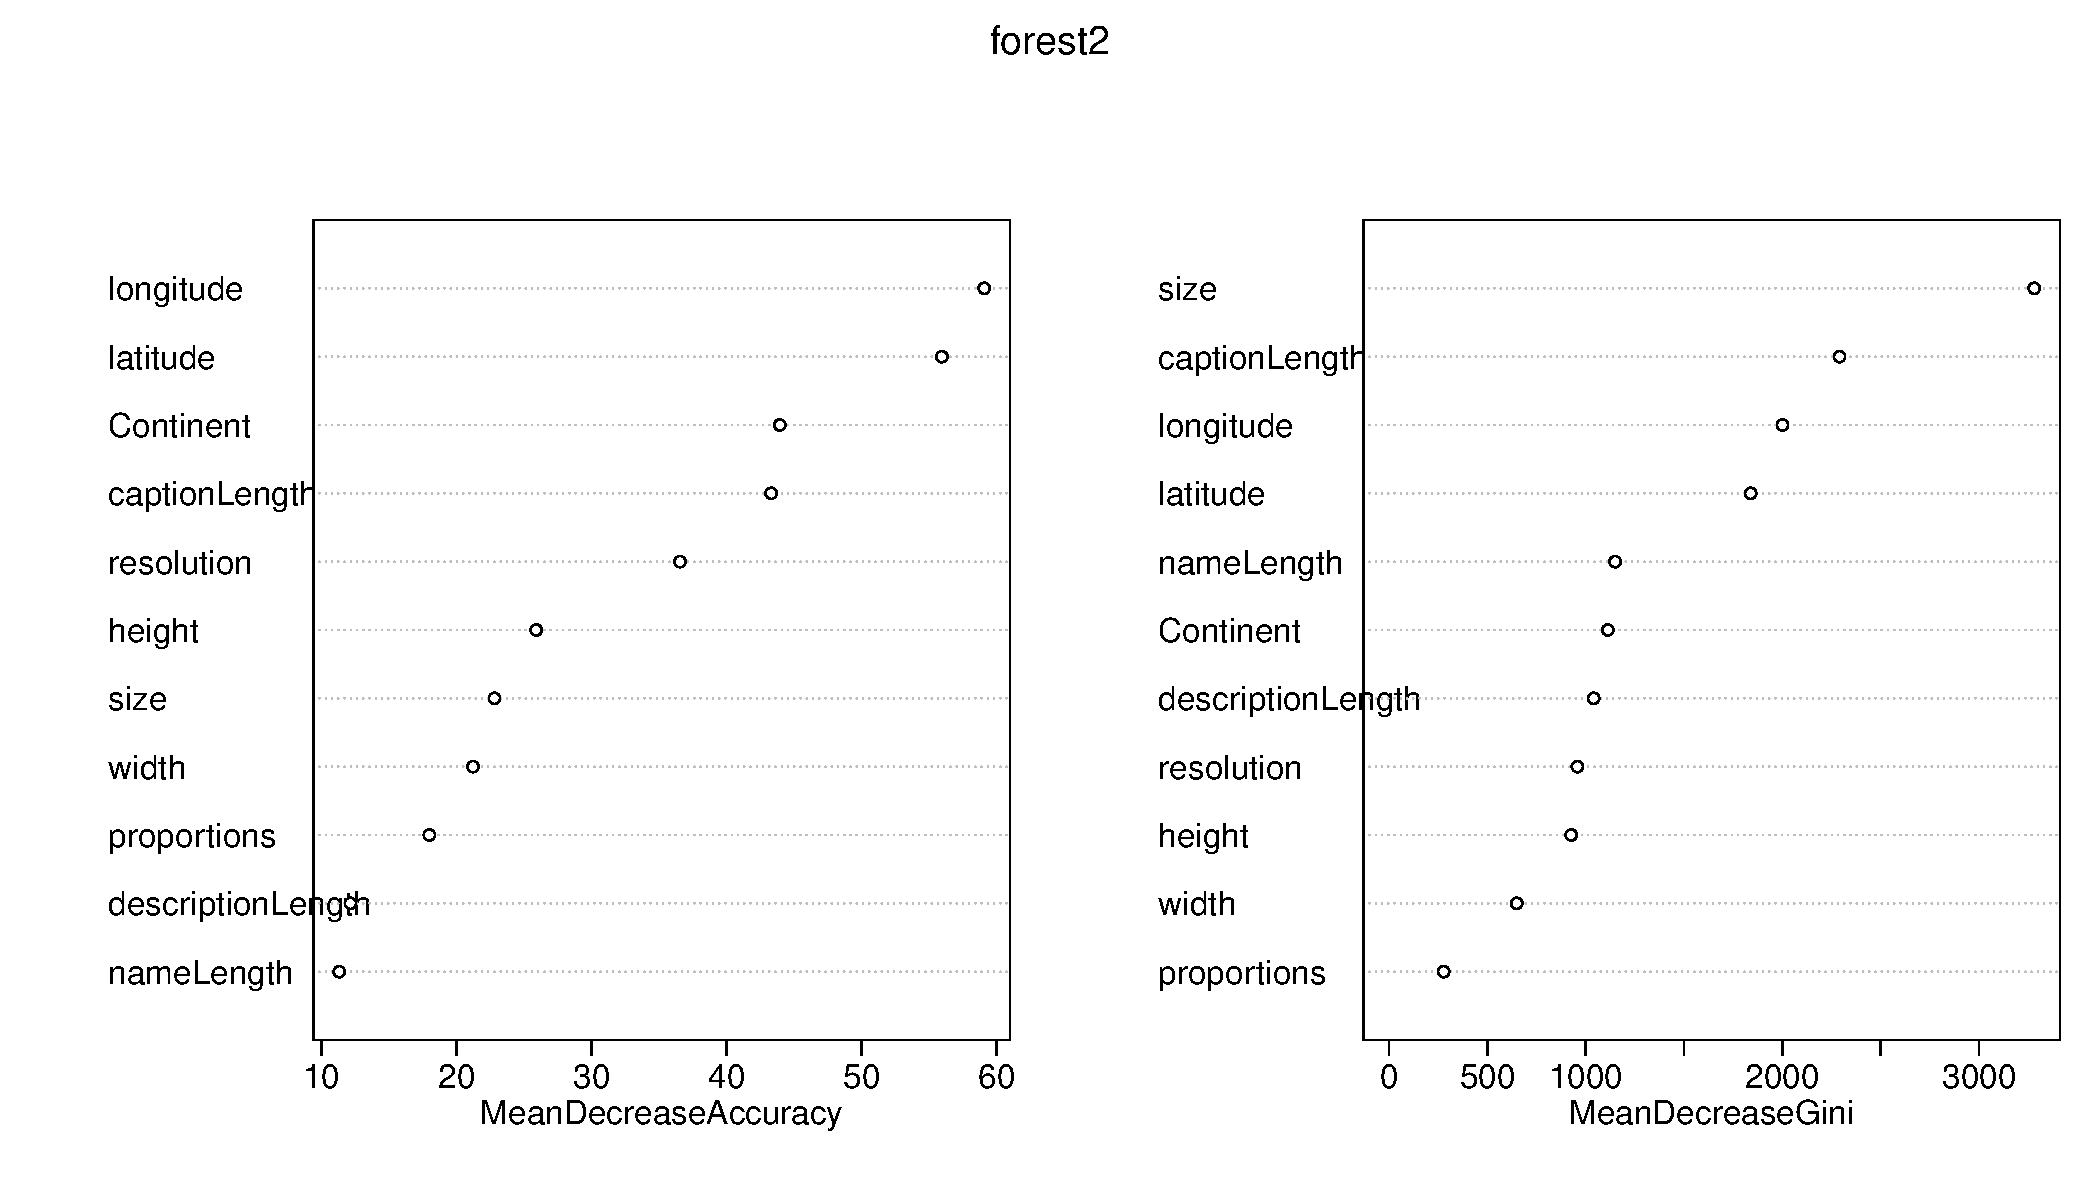
\includegraphics[width=1\textwidth]{./img/Rplot03.pdf}
	\caption{Dane wygenerowane przez pakiet "randomForest"}
\end{figure}

\newpage

Graf po lewej oznacza, jak wielki wpływ miał dany atrybut - przede wszystkim jak wysoko wykonywany był rozłam na jego podstawie (im wyżej, tym większy wpływ na kształt drzewa miał). Graf po prawej określa rozdrobnienie, czyli jak często dokonywano rozłamów (niekoniecznie w górnej części drzewa).

\section{Wnioski i podsumowanie}

W trakcie testów aplikacji otrzymywaliśmy wyniki w okolicach 16-18\% albumów dobrych jakościowo dla algorytmu drugiego (randomForest) i około 14-15\% dla algorytmu pierwszego (cforest z pakietu "party"). Są to wartości zbliżone do proporcji z zestawu treningowego. Należy jednak zaznaczyć, że w przypadku pierwszego algorytmu pamięć przydzielona przez R.NET została wyczerpana i niemożliwe było dokończenie obliczeń. Z tego powodu, predykcja za pomocą funkcji cforest była jedynie na połowie zestawu treningowego (około 20000 wierszy). \\

W trakcie testów zmieniano ilość podawanych atrybutów podawanych w formule. Okazało się, że najlepsze wyniki uzyskuje się wykorzystując wszystkie z nich - algorytm lasów sam dobiera sobie, które są dla niego atrakcyjniesze, a mniej ważne są rzadziej używane. W naszym przypadku było to w sumie 11 kolumn: długość i szerokość geograficzna, kontynent, wysokość i szerokość zdjęcia, proporcje, przekątna, ilość zdjęć w albumie oraz długość (w słowach) nazwy, opisu i podpisu albumu. Pomijając formułe, ważne znaczenie miały 2 parametry:

\begin{itemize}
	\item \textbf{mtry} - określa, ile atrybutów z kolumny będzie losowanych podczas tworzenia lasu.
	\item \textbf{ntree} - ilość drzew w lesie.
\end{itemize}

Szybko okazało się, że najlepszą wartością dla parametru mtry jest ta domyślna - pierwiastek kwadratowy z 11, co po obliczeniu sufituu dawało 4 losowe atrybuty spośród wszystkich 11. Mniejsza ilość sprawiała, że predykcja była niezbyt dokładna, natomiast większa powodowała zjawisko podobne do overfittingu. Nieco inaczej sytuacja wyglądała w przypadku ilości drzew, gdzie nie udało się stwierdzić aż takiej zależności.  Przy bardzo małych wartościach (np. mniej niż liczba losowanych atrybutów) wyniki były niezbyt dokładne, już przy 10 stabilizowały się na pewnym poziomie, natomiast po osiągnięciu pewnego pułapu (więcej niż 200 drzew) nie różnice stawały się niezauważalne (trzeci rząd po przecinku). Wybór ilości drzew oddaliśmy do dsypozycji użytkownikowi aplikacji.\\

W międzyczasie próbowaliśmy zrealizować zadanie poprzez użycie sieci neuronowych (pakiet "neuralnet"), co jednak się nie udało - małe sieci po długim czasie wykonywania (około 5-10 minut) dawały niezadowalające wyniki, natomiast te bardziej rozbudowane wykonywały się ponad 2 godziny (dokładny czas nieznany). Po sprawdzeniu tendencji na stronie kaggle.com okazało się, że do zadań podobnych do naszego sieci neuronowe są stosunkowo rzadko wykorzystywane.\\

Projekt z przedmiotu Biologicznie Inspirowane Systemy Sztucznej Inteligencji był jednym z najciekawszych inicjatyw na naszych studiach. Interesująca tematyka oraz nowoczesne rozwiązania z dziedziny machine learningu sprawiły, że podeszliśmy do zagadnienia ambitniej niż do nudnego obowiązku. Mieliśmy okazję zapoznać się z potężnym narzędziem, jakim jest język programistyczny do analizy danych statystycznych R. W trakcie programowania okazało się, że fragment aplikacji pisany w C\# jest w zasadzie niepotrzebny - używany był jedynie do stworzenia przyjemnego dla oka interfejsu użytkownika, podczas gdy właściwą wartością merytoryczną aplikacji był wygenerowany przez nią zbiór wynikowy. Żałujemy jedynie, że nie mogliśmy zaprezentować naszych wyników na stronie kaggle.com, aby uzyskać konkretniejsze dane na temat poprawności predykcji, a może nawet zdobyć jakąś nagrodę.

\theendnotes

\end{document}